\todo{prendre en compte remarques de JMR dans mail}

\label{lab:chapPET}
La Tomographie par \'Emission de Positons (TEP) est une modalité d'imagerie fonctionnelle utilisant la désintégration d'un traceur radioactif pour mettre en valeur les zones de forte activité métabolique. Elle est principalement utilisée en imagerie cérébrale, oncologique et cardiologique.

Le traceur $^{18}FDG$ est un traceur analogue du glucose utilisé en oncologie.

Dans ces trois chapitres, nous allons tout d'abord détailler rapidement les principes physiques amenant à la création des images TEP, de la désintégration du traceur radioactif à la détection des photons émis lorsqu'ils atteignent un capteur. Ensuite, nous parlerons des solutions techniques mises en place pour réaliser les images TEP, avec les différents types d'acquisitions. Enfin, nous détaillerons les algorithmes utilisés pour reconstruire les images TEP.

 
\chapter{Principe Physique}

	\section{Généralités}

L'imagerie TEP permet de visualiser de manière indirecte des processus physiologiques survenant dans le corps du patient. Je vais présenter rapidement les évènements qui se produisent lors d'un examen, présentés dans la figure~\ref{fig:schemaTEP}.

Pour cela, on lui injecte un ``traceur'' contenant une particule radioactive. Ce traceur est conçu de manière à se fixer sur les zones du corps que l'on souhaite imager. Pendant toute la durée de l'examen, les particules radioactives vont se désintégrer selon la loi de décroissance radioactive de l'équation~\ref{eq:loidecradioact}.

\begin{equation}
	dN = - \lambda N dt
	\label{eq:loidecradioact}
\end{equation}

$N$ représente le nombre de particules radioactives présentes dans le corps du patient. $dN$ représente la variation de ce nombre de particules (le nombre de désintégrations par $dt$) et $\lambda$ est une constante dépendant de l'élément radioactif.

Chaque désintégration d'un élément radioactif va déclencher l'émission d'une particule chargée $\beta^+$, aussi appelée positon. En oncologie, on utilise le Fluor $^{18}F$ qui se désintègre en Oxygène $^{18}O$ en émettant le positon. Cette particule va parcourir quelques mm avant de s'annihiler avec un électron en émettant 2 photons dans deux directions opposées avec une énergie de 511 KeV.

Ce sont ces photons qui sont détectés par l'imageur TEP. Ils représentent une coïncidence, car l'instant d'arrivée et leur énergie sont semblables. L'ensemble des ``Lignes de réponse'' (LDR) correspondant aux coïncidences détectées est utilisée pour reconstruire les images.

\begin{figure}
\centering
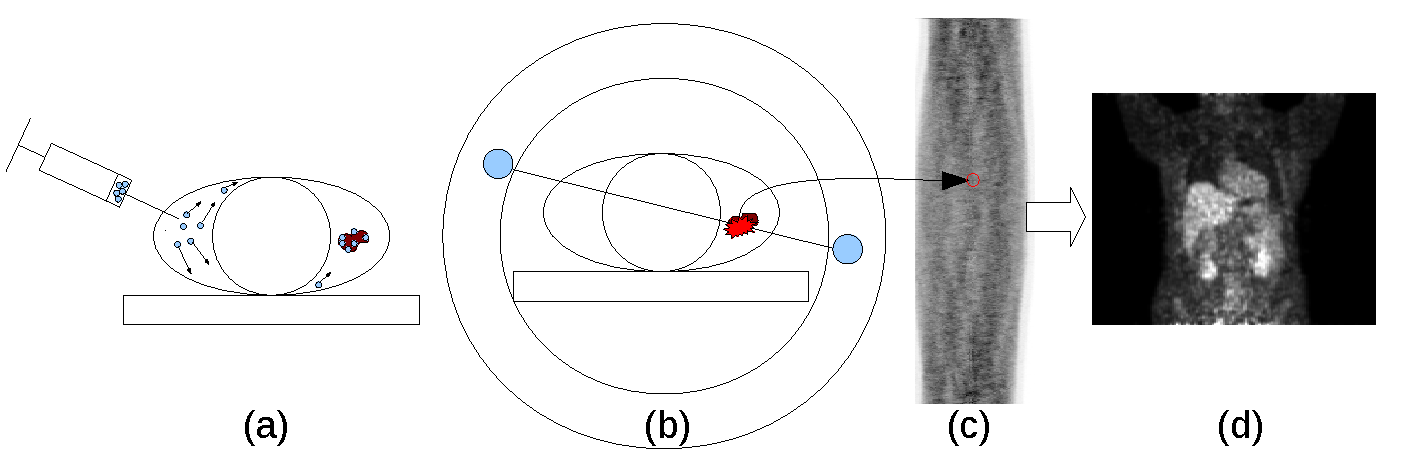
\includegraphics[width=16cm]{images/schemaTEP}
\caption[Présentation simplifiée de la TEP]{Processus d'un examen TEP : a) Injection du traceur radioactif, qui va se fixer préférentiellement sur les zones que l'on cherche à observer. b) Désintégration d'un atome radioactif du traceur, ici dans la zone à imager. Cela entraîne l'émission de deux photons dans deux directions opposées, qui seront détectés dans la couronne de capteurs. c) Tous les évènements détectés sont stockés dans la mémoire de la console, ici sous forme de sinogramme. d) L'image est reconstruite à la suite de l'acquisition pour former un volume 3D estimant la répartition du traceur dans l'organisme.}
\label{fig:schemaTEP}
\end{figure}


\section{Traceur $^{18}$FDG}

Le glucose est considéré comme un carburant essentiel à l’organisme qui peut l’assimiler directement. Les cellules cancéreuses, qui ont un métabolisme accéléré par rapport aux autres cellules du milieu, sont particulièrement friandes de glucose. Celui-ci est transporté à l’intérieur des cellules par des transporteurs spécifiques de la membrane afin d’être dégradé par un ensemble de réactions appelé glycolyse. Le glucose est d’abord phosphorylé en glucose-6-phosphate, catalysé par l’enzyme hexokinase. Le glucose-6-phosphate est ensuite transformé en fructose-6-phosphate qui subit à son tour plusieurs transformations successives pour être finalement excrété par la cellule sous forme de lactate.

Le fluorodeoxyglucose ou FDG est un analogue du glucose avec un aspect structural très proche. Il est donc aussi capté par les cellules, mais ne peut pas être utilisé dans leur métabolisme. Le FDG suit le même processus métabolique que le glucose jusqu’à l’étape de phosphorylation en FDG-6-phosphate. Il n’est cependant pas métabolisé par l’enzyme glucose-6-phosphatas et s’accumule donc dans la cellule sous la forme de FDG-6-phosphate. Cette accumulation permet de distinguer la présence de tumeurs, généralement beaucoup plus gourmandes en énergie que les tissus sains et donc marquées par une présence élevée de FDG-6-phosphate. Par son métabolisme et son importance pour les cellules cancéreuses, le FDG est donc actuellement préconisé en clinique pour les examens concernant des patients en cancérologie. Il est généralement marqué au fluor 18 donnant le $^{18}$FDG.

Cependant, ce radiotraceur n'est pas spécifique aux tumeurs mais se fixe sur toute cellule consommant du glucose. C'est pourquoi le coeur ainsi que le cerveau fixent toujours une grande quantité de $^{18}FDG.

\section{\'Emission des photons}

Nous allons maintenant détailler le processus qui déclenche l'émission des photons détectés par l'imageur, présenté dans la figure~\ref{fig:Langner2008ad}.

Les émetteurs de positons utilisés en TEP sont des isotopes radioactifs présentant un excès de charge positive, ou proton, dans leurs noyaux. Un processus de désintégration $\beta^+$, correspondant à la transformation d’un proton $p$ en un neutron $n$, leur permet de migrer vers un état stable. Cette désintégration résulte en l’émission d’un neutrino $\nu$ et d’un positon $e^+$ selon l’équation~\ref{eq:desinteg}. Le positon est une particule de même masse que l’électron mais de charge opposée.

\begin{equation}
 p~\rightarrow~n + e^+ + \nu
\label{eq:desinteg}
\end{equation}

Le positon va alors s'annihiler avec un électron après un parcours de quelques millimètres en émettant simultanément deux photons de même énergie (511 keV) comme indiqué dans l'équation~\ref{eq:annihilation}. L'angle d'émission des photons est de $180°$ avec une incertitude de $\pm 0.25°$~\cite{bailey2005positon}.

\begin{equation}
 e^+ + e^-~\rightarrow~\gamma + \gamma
\label{eq:annihilation}
\end{equation}

\begin{figure}
\centering
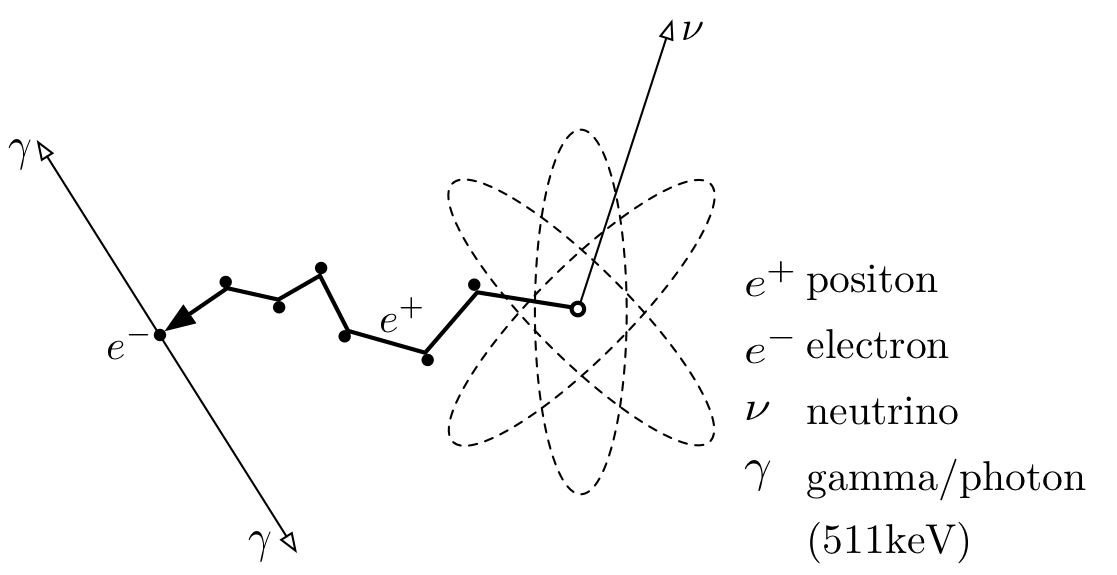
\includegraphics[width=12cm]{images/annihilation}
\caption[\'Emission des photons]{\'Emission des photons~\cite{Langner2008ad} : Le radio traceur se désintègre en émettant un neutrino et un positon. Après un parcours de quelques mm dans les tissus, ce dernier s'annihile avec un électron. Cette réaction provoque la création de deux photons d'énergie 511 keV partant dans deux directions opposées.}
\label{fig:Langner2008ad}
\end{figure}

\section{Détection des photons}

Les détecteurs utilisés en TEP sont constitués d'un couplage entre un cristal et un tube photomultiplicateur, le tout placé devant un photodetecteur. Chaque photon absorbé par le matériau photomultiplicateur va entraîner une réaction en chaîne qui va déclencher une émission lumineuse. Le capteur situé derrière va convertir cette émission lumineuse en charge électrique. Habituellement,  

Un système électronique va ensuite apparier les photons détectés pour retrouver la ligne de réponse (LDR) sur laquelle la désintégration a eu lieu. Les paires de photon assemblées correspondent à des coïncidences.

Les détecteurs sont regroupés par blocs, placés en anneaux autour du patient. L'imageur TEP Gemini que nous utiliserons dans cette étude dispose de 28 blocs, contenant chacun une matrice de 29 par 22 cristaux de GSO. Une photo de l'imageur ouvert est visible en~\ref{fig:gemini_ecl}. 420 Photomultiplicateurs placés autour des blocs sont utilisée pour estimer la position des détections.

\todo{préciser, ajouter images (thèse sandrine ?)}

\begin{figure}
\centering
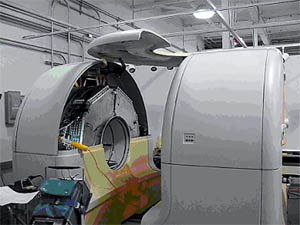
\includegraphics[width=12cm]{images/gemini_eclate}
\caption[Photo d'un imageur philips Gemini ouvert]{Cette photo représente la partie PET d'un imageur Philips Gemini ouverte. On distingue nettement les cartes électroniques connectées aux tubes photomultiplicateurs.}
\label{fig:gemini_ecl}
\end{figure}

	\section{Types de coïncidences}

La figure~\ref{fig:schemaDetections} représente les différents types de coïncidences rencontrés en TEP.

Les coïncidences vraies (\ref{fig:schemaDetections}.a) correspondent aux cas où les deux détections appariées correspondent bien à une seule désintégration et où aucun des photons n'a été dévié. Les coïncidences fortuites (\ref{fig:schemaDetections}.b) correspondent à la détectio nen coïncidence de deux photons issus de deux annihilations différentes, par exemple à cause de l’absorption d’un des photons d’une désintégration par les tissus. Enfin, les coïncidences diffusées (\ref{fig:schemaDetections}.c) sont le résultat de la déviation d'un des deux photons produit engendré par des interactions rayonnement-matière dans les tissus (diffusion compton). Pour éliminer ces erreurs, un certain nombre de méthodes ont été implémentées, dont le filtrage en énergie et en temps au niveau matériel : ne sont prises en compte que les paires d'évènements arrivant dans une fenêtre temporelle et énergétique définie. En effet, les photons déviés vont perdre de l'énergie, ce qui va entraîner leur élimination.

Les coïncidences diffusées ainsi que les coïncidences aléatoires génèrent un bruit parasite dans les sinogrammes. L'absorption des photons sans détection va engendree un effet d'atténuation du signal qui sera de plus en plus important en fonctio nde la profondeur des tissus et de leur absorption.


\begin{figure}
\centering
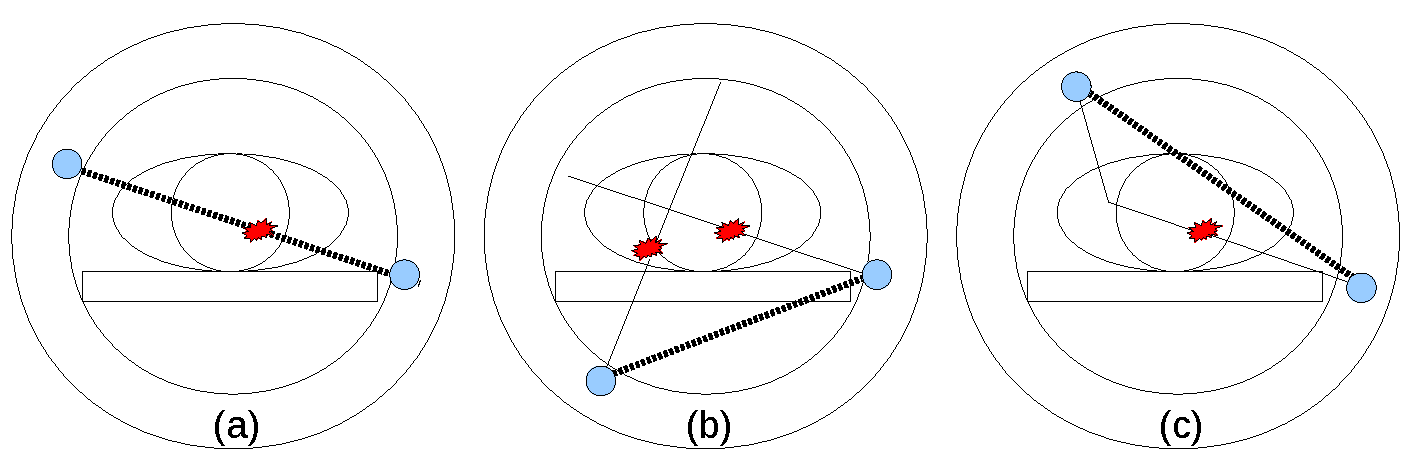
\includegraphics[width=12cm]{images/schemaDetections}
\caption[Les différents types de coïncidences en TEP]{Les différents types de coïncidences en TEP. Le trajet réel du photon est indiqué en trait fin simple, tandis que la ligne de réponse est indiquée en trait pointillé épais. On appelle les coïncidences vraies (a) lorsque l'annihilation est bien sur la ligne de réponse, fortuites (b) lorsque deux désintégrations réalisées en même temps sont considérées comme une seule et diffusée (c) lorsqu'un des photons est dévié.}
\label{fig:schemaDetections}
\end{figure}



	\section{Perturbation du trajet du photon}

Les deux interactions les plus importantes que peuvent avoir les photons avec les tissus sont la diffusion compton et l'absorption photoélectrique. L'effet Rayleigh, qui correspond à la diffusion du photon sur un atome, est peu présent aux énergies concernées par la TEP. 

La diffusion compton correspond à l'interaction entre le photon émis et un électron du milieu. L'énergie cinétique de l'électron est augmentée, tandis que le photon est dévié. Il est intéressant de noter qu'une déviation de 25° engendre une perte d'énergie du photon de seulement 10\%~\cite{evans1955atomic}.

L'absorption photo-électrique correspond quand à elle à l'interaction entre un noyau atomique et un des photons. L'énergie du photon est absorbée par le noyau et transmis à un de ses électrons. 

L'atténuation du signal est lié à une combinaison de ces effets. Tout ce qui peut perturber le trajet du photon et perturber sa détection. L'effet d'aténuation est particulièrement important en TEP, car il génère des artefacts très visibles, qui doivent être corrigés à partir d'une carte d'atténuation, déduite d'un examen de Tomodensitométrie (Tomographie par rayons X) ou d'une carte de transmission, comme indiqué en~\ref{fig:schemaAtt}.

\todo{citer des publis pour les 3 effets !}

On peut représenter cette atténuation de manière analytique à l'aide de la loi de Beer-Lambert, qui montre que l'atténuation augmente exponentiellement avec la longueur du trajet dans les tissus :
\begin{equation}
I = I_0 e^{-\mu l}
\end{equation}

Avec $I_0$ la quantité originale de photons, $I$ le nombre de photons qui traversent le milieu, $\mu$ le coefficient d'atténuation du milieu et $l$ la longueur du trajet. 

Dans le cas où le milieu est complexe, et si l'on connaît l'atténuation $\mu(x)$ en chaque point $x$ du trajet, on peut connaître précisément l'atténuation subie selon chaque ligne de réponse :

\begin{equation}
I = I_0 e^{- \int\limits^L_0 \mu(l) dl}
\end{equation}


\begin{figure}
\centering
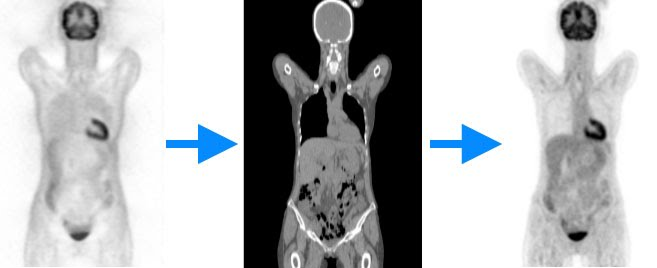
\includegraphics[width=12cm]{images/attenuationNonAtt}
\caption[Effet de l'atténuation sur les images TEP]{Effets de l'atténuation sur des images TEP : L'image de gauche correspond à la distribution de radioactivité reçue par les détecteurs. On peu observer une perte progressive de l'activité vers l'intérieur des tissus, car les photons ont plus de chances d'interagir avec la matière. L'image TDM au centre est utilisée pour estimer une carte de l'atténuation des tissus et prendre en compte cette atténuation lors de la reconstruction de l'image TEP.}
\label{fig:schemaAtt}
\end{figure}

\section{Quantification en imagerie}

L'image visualisée par le clinitien est directement liée à  la concentration de lisotope radioactif du fluor, le $^{18}F$. La concentration observée est la somme des isotope piégés dans les cellules et des isotopes libres dans le système vasculaire. Cependant, cette concentration mesurée est très dépendante du volume du patient, ainsi de de la dose injectée.

En clinique, on utilise habituellement le SUV (Standard Uptake Value), qui corresponds à une tentative de fournir des valeurs indépendantes de la dose injectée et du patient. Cela permet de réaliser des comparaisons entre des fixations radioactives de plusieurs examens, voir de plusieurs patients.

Le SUV est défini comme suit :

\begin{equation}
SUV=\frac{C}{ \frac{dose inject\acute{e}e}{poids corporel} }
\end{equation}

\todo{vérifier que c'est bien passé}

\chapter{Déroulement d'une acquisition}


Nous allons maintenant décrire rapidement quelques points techniques permettant de mieux comprendre comment sont réalisées les acquisitions. Nous parlerons de la méthode utilisée pour réaliser des acquisitions corps entier alors que l'imageur a un champ de vue axial limité et des contraintes associées. Enfin nous aborderons la problématique du format des données ses implications.

\section{TEP au $^{18}$FDG}


En oncologie, les patients qui ont une suspicion de cancer se voient proposer un examen TEP pour réaliser un diagnostic initial, qu iva viser à déterminer le degré de malignité de la pathologie détectée. Il a été montré~\cite{gould2001accuracy} que les performances de la TEP sur la détection des lésions pulmonaires étaient supérieur à l'imagerie anatomique. Les performances de la TEP sont aussi reconnues pour les cancer hépatiques et la détection précoce des lymphomes. Plusieurs images sont visibles dans la figure~\ref{fig:exTEP}.

La TEP est ensuite utilisé pour suivre l'évolution des lésions, afin d'adapter le traitement à l'évolution de la maladie.

\begin{figure}[h!]
\begin{center}
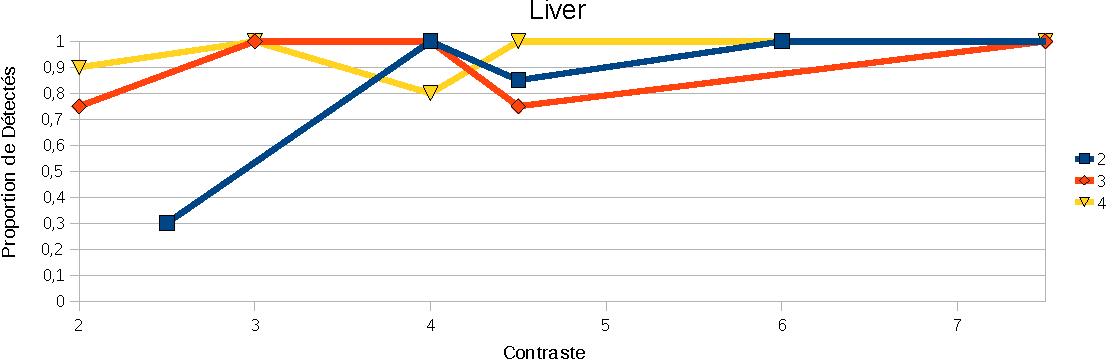
\includegraphics[width=15cm]{images/calibrationFoie_crop}
\end{center}
\caption{Exemples d'images } 
\label{fig:exTEP}
\end{figure}

\todo{ajouter les exemples d'images}

\section{Acquisitions corps entier}


Les acquisitions TEP réalisées pour l'oncologie sont habituellement des acquisitions corps entier, de manière à pouvoir avoir une vue de l'étendue des lésions.

Or le champ de vue axial de la plupart des caméras TEP est de l'ordre de 15 à 20 cm environ (18 cm pour le Philips Gemini GXL). En routine clinique, le patient est placé sur un lit qui se déplace par incréments successifs lors de l'acquisition.

Le nombre de positions lits est déterminé par la taille du patient ainsi que par le champ de vue du tomographe. Chaque lit est reconstruit séparément puis assemblé avec les lits suivants et précédents, comme indiqué dans la figure~\ref{fig:multilits}. \'Etant donné que les caméras TEP ont une sensibilité plus faible à leurs extrémités, on introduit un chevauchement plus ou moins important dans les lits.

\begin{figure}
\centering
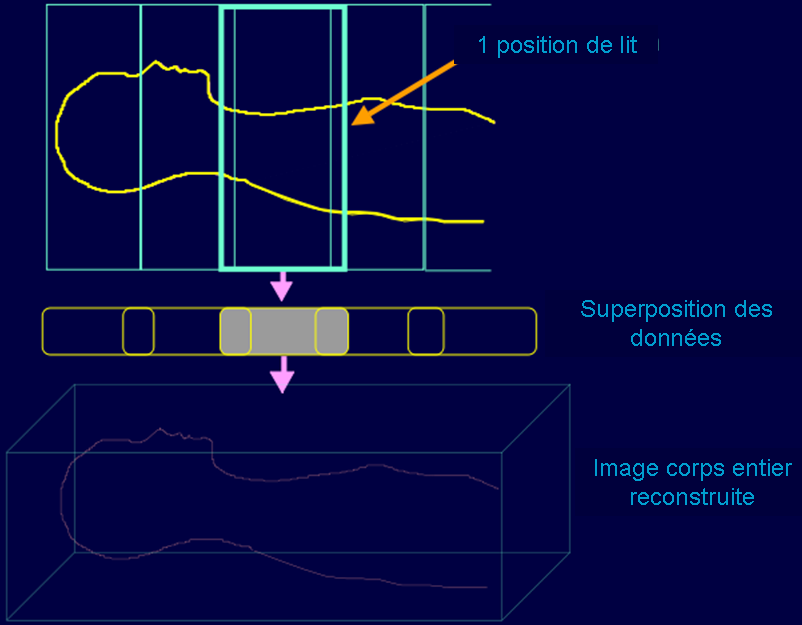
\includegraphics[width=12cm]{images/multilits}
\caption[Acquisitions corps entier en TEP]{Réalisation d'une acquisition corps entier en TEP : Chaque lit est acquis et reconstruit séparément avec un chevauchement. Les lits sont ensuite assemblés pour produire l'image finale.}
\label{fig:multilits}
\end{figure}

\todo{combien de lits cam' philips ?}

Les acquisitions corps entier utilisent typiquement plus de 10 lits sur la caméra philips Gemini, ce qui demande un temps considérable. Il faut donc faire des compromis entre le temps d'acquisition et la qualité des images. Sachant que les examens TEP sont coûteux et que l'immobilité est inconfortable pour les patients, le temps d'acquisition est calibré pour durer moins d'une heure au total. Les nouvelles générations d'imageurs permettent cependant de réduire les temps d'acquisition à 2 minutes par lit à qualité équivalente.


	\section{Acquisition en mode 3D}

Historiquement, les données étaient acquises par coupe : des septas (plaque destinées à absorber les photons) étaient placés entre les détecteurs de manière à éliminer les photons qui n'étaient pas émis dans le plan (voir figure~\ref{fig:2D3D}). 

Aujourd'hui, la totalité des scanners fonctionnent en mode 3D uniquement. Le retrait des septa permet d'augmenter le rapport signal sur bruit pour les gammes d'activité injecté aux patients, même si la détection des coïncidences vraies s'accompagne d'une augmentation de bruit parasite lié à l'augmentation de la détecti ondes coïncidences fortuites.


\todo{mettre illustration camera philips gemini - virer partie 2D}

\begin{figure}
\centering
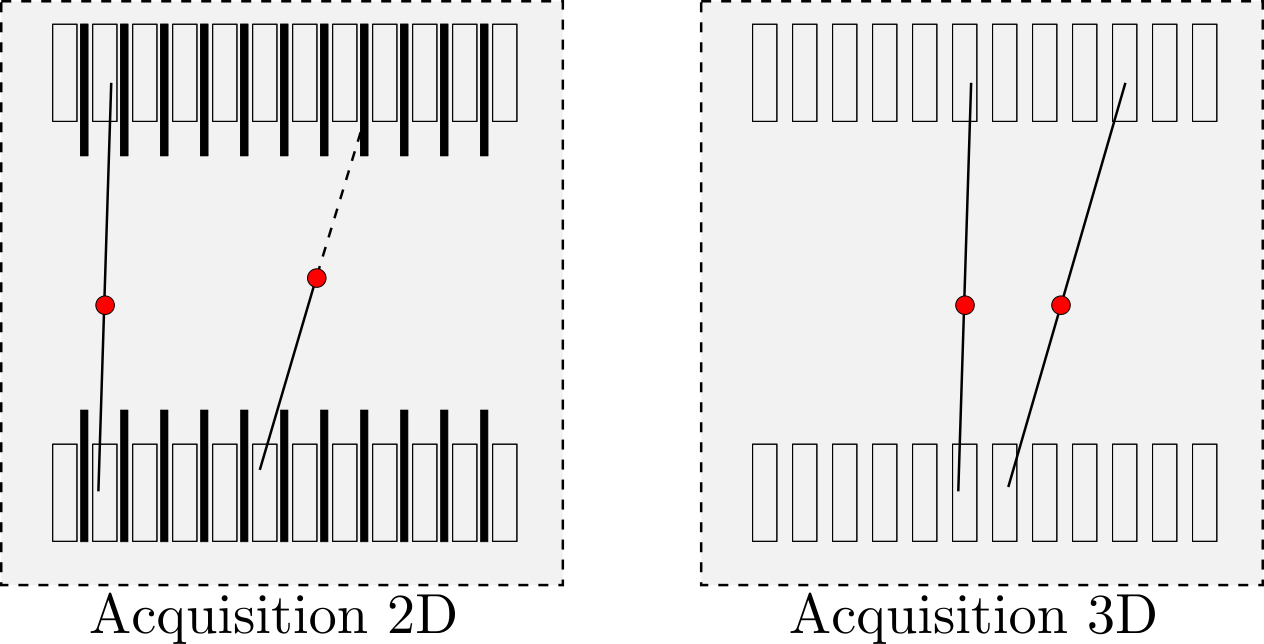
\includegraphics[width=12cm]{images/2D3D}
\caption[Acquisitions 2D et 3D en TEP]{Illustration des différences entre l'acquisition 2D et 3D en TEP. Les deux images représentent un imageur vu en coupe axiale. Les rectangles blancs représentent les détecteurs et les rectangles noirs les septas destinés à bloquer les photons. }
\label{fig:2D3D}
\end{figure}


%	\section{Corrections}

	\section{Correction de l'atténuation}
\label{CorrectionAttenuation}

Le patient passe tout d'abord un examen TDM sur les scanners couplés TEP/TDM. Les valeurs des coefficients Hounsfield correspondant à l'atténuation des rayons X sont transformés pour correspondre à l'atténuation des photons de 511keV de la TEP. Cette image est ensuite utilisée pour réaliser la correction d'atténuation. 

Une technique plus ancienne d'estimation de la carte d'atténuation est basée sur une image acquise en transmission, où une source radioactive émettrice de positon est placée dans l'imageur et tourne autour du patient. Une acquisition  préalable est réalisée ``à blanc'', sans le patient. Le rapport entre la quantité de photons reçue par les détecteurs avec et sans le patient permet de générer la carte d'atténuation du corps du patient, de la même manière que pour l'imagerie TDM. Cependant, la généralisation des scanner couplées TEP/TDM limite l'utilisation de cette technique.

\begin{equation}
I(x) = I_0(x) e^{-\mu x}
\end{equation}

En connaissant la radioactivité reçu sans le patient (à blanc") $I_0$, la radioactivité reçue avec le patient $I$, on peut en déduire la valeur de $\mu$.

%\subsection{Correction des coïncidences fortuites}

%Des techniques existent pour corriger les données des effets vus dans la figure~\ref{fig:schemaDetections}, notamment l'implantation d'une ligne à retard pour estimer les coïncidences aléatoires puis les retirer du sinogramme.


	\section{Format des données}
Les données acquises par une caméra TEP peuvent être stockées sous deux formes principales : séquentiel et sinogramme.

		\subsection{Séquentiel}
\label{lab:modeliste}
Ce format correspond à un enregistrement ``brut'' des données issues de l'électronique de la caméra. Il est aussi appellé mode liste.

Ce format de fichier est en fait un enregistrement séquentiel des évènements, dans leur ordre de détection. On peut enregistrer chaque photon détecté indépendamment, ou encore uniquement les coïncidences. Chaque évènement est daté, ce qui permet de conserver l’information temporelle, qui est utilisé notamment pour synchroniser les données acquises avec le temps, pour la correction de mouvement par exemple, ou pour observer comment se répartit le radio-traceur au cours du temps.

Il existe plusieurs formats publiques de fichiers pour le stockage de ces données, notamment le format LMF (List-Mode Format) développé pour le projet ClearPET et le format ROOT développé par le CERN. Cependant, chaque constructeur utilise son propre format de fichier propriétaire.


Cependant, ce format consomme une très grande quantité de ressources, étant donné qu'un examen PET est constitué de plusieurs millions d'évènements. Cela engendre de fortes contraintes en espace disque et complique de beaucoup la manipulation des données. 

		\subsection{Sinogramme}

Le sinogramme est une matrice indiquant pour chaque ligne de réponse le nombre de détections réalisées, comme présenté dans la figure~\ref{fig:sino}. En ordonnés sont représentés les angles de la ligne de réponse, et en abscisse leur distance au centre du détecteur~\cite{fahey2002data}. Dans le mode 3D, on détecte des paires de photon qui ne sont pas directement dans le plan du détecteur. Une dimension supplémentaire est donc nécessaire ajoutée pour prendre en compte cet effet.

Le principal avantage du sinogramme est qu'il permet de stocker les données acquises lors d'un examen TEP de manière beaucoup plus compacte que le format séquentiel. Cependant, il ne conserve aucune information temporelle.

\begin{figure}
\centering
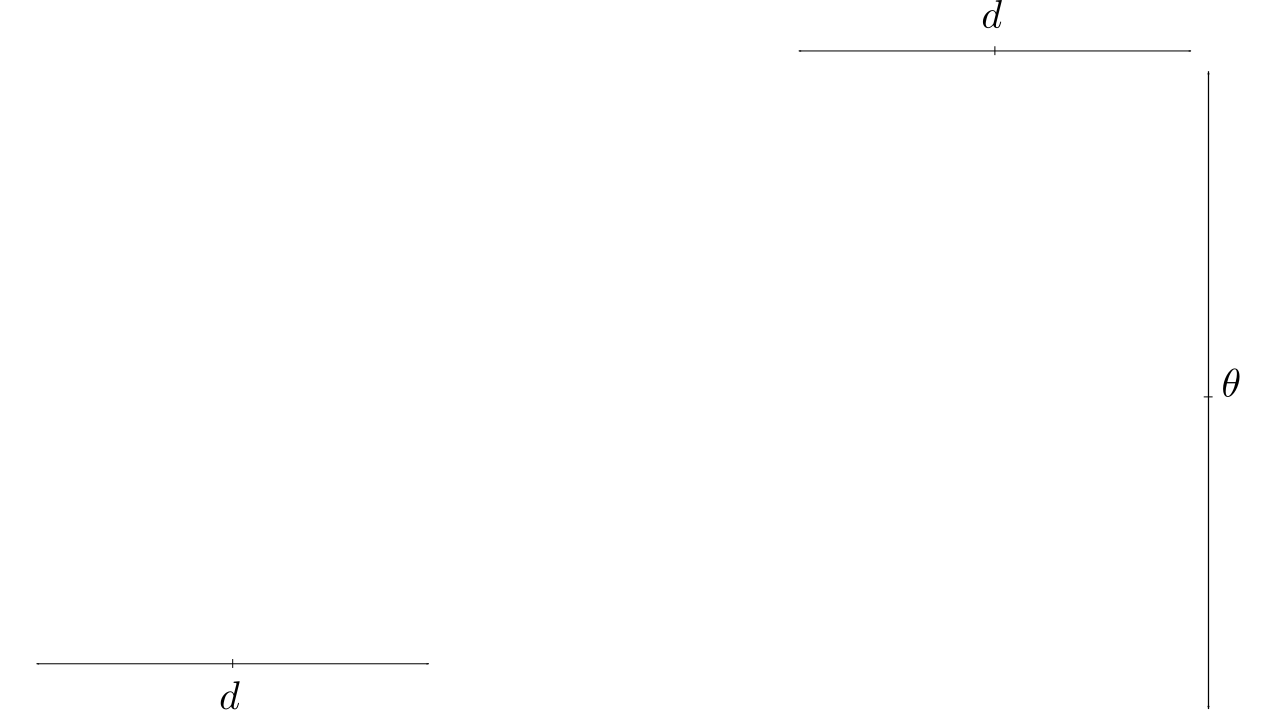
\includegraphics[width=11cm]{images/sino}
\caption[Principe du sinogramme]{Exemple de sinogramme: chaque ligne corresponds à une projection de l'image selon un angle $\theta$ correspondant à la position de la ligne dans le sinogramme.}
\label{fig:sino}
\end{figure}


\chapter{Algorithmes de reconstruction}

La reconstruction des images TEP correspond à un problème inverse : à partir de l'ensemble des lignes de réponse, il faut déduire la répartition du radio traceur dans l'organisme du patient. Deux classes d'algorithme existent pour résoudre ce type de problèmes, mais actuellement seuls les algorithmes itératifs sont utilisés en oncologie clinique. 

	\section{Algorithmes Itératifs}

La relation liant l'image TEP $f$ et les projections sur les détecteurs $p$ est la suivante :

\begin{equation}
	p = R f + e
\label{eq:eqTEP}
\end{equation}

Avec $R$ la matrice de projection et $e$ correspondant aux phénomènes parasites. On considère que les comptages des lignes de réponses $p_i$ sont indépendants et bruités selon une loi de poisson. Ce problème est mal posé, et nécessite donc l'utilisation d'algorithmes spécialisés. 


		\subsection{Algorithme ML-EM (Maximum Likelihood Expectation Maximisation) }


L'algorithme ML-EM~\cite{shepp1982maximum} est initialisé avec une image de départ $f_0$. Il se déroule en deux phases principales : une phase de comparaison de l'image au niveau $n$ avec les lignes de réponses observées, puis une phase de mise à jour de l'image pour prendre en compte les différences calculées à l'étape précédente, comme présenté dans la figure~\ref{fig:schemaMLEM}.


\todo{introduire concept de vraisemblance pour amener à l'équation}
L'équation correspondant à ML-EM est la suivante :

\begin{equation}
	f_j^{(n+1)}=\frac{\hat{f}_j^{(n)}}{\sum\limits_{i'}H_{i'j}}\sum\limits_{i}H_{ij}\frac{p_i}{\sum\limits_{k}H_{ik}\hat{f}_k^{(n)}}
\label{eq:MLEM}
\end{equation}

En pratique, la matrice système $H$ correspond à la matrice de projection $R$ présentée dans l'équation~\ref{eq:eqTEP} mais inclus des informations supplémentaires pour corriger les différences de sensibilité entre les différents capteurs, et réaliser la correction des diffusés~\cite{shepp1982maximum,chornoboy1990evaluation}. Cette matrice peut aussi être utilisée pour corriger l'atténuation des tissus. En pratique, cette matrice ``système'' $H_{ij}$ indique la probabilité de détecter une désintégration issue du voxel $j$ de l'image dans la ligne de réponse $i$.




Le nombre d'itérations à réaliser avant d'atteindre la convergence dépend de l'image, mais il est couramment d'environ 20 à 50. Il existe plusieurs publications proposant un critère d'arrêt~\cite{bissantz2006multi}, mais en pratique la reconstruction est souvent réalisée pour un nombre d'itérations fixées~\cite{bailey2005positon} et  suivi d'un filtrage passe-bas~\cite{daube2001application}. Cet algorithme de reconstruction prend un temps important car il faut réaliser l'opération de projection et de rétroprojection sur l'ensemble des données à chaque itération.

\begin{figure}
\centering
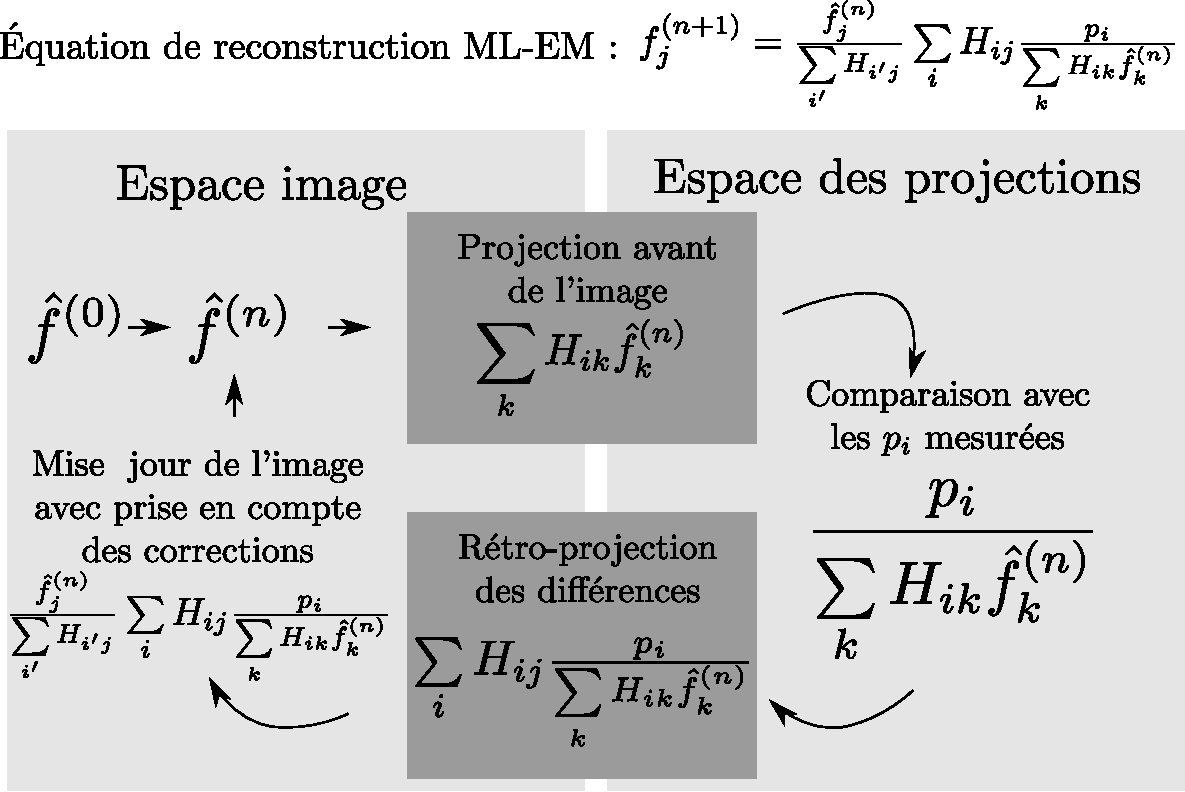
\includegraphics[width=12cm]{images/MLEM}
\caption[Schéma de principe de l'algorithme MLEM]{Schéma décrivant l'algorithme itératif ML-EM. $\hat{f}^{(n)}_j$ est l'estimation du voxel $j$ de l'image à l'itération $n$. $H_{ij}$ est la matrice système, et représente la probabilité de détecter une désintégration dans le voxel $j$ à la ligne de réponse $i$.}
\label{fig:schemaMLEM}
\end{figure}


	\subsection{Algorithme OM-EM (Ordered Subset Expectation Maximisation)}

L'algorithme OS-EM est une évolution de l'algorithme ML-EM  qui permet une accélération substantielle de la convergence en réalisant les itérations de l'équation~\ref{eq:MLEM} sur des sous-ensemble des données acquises~\cite{hudson1994accelerated}. 

Ces sous-ensemble de données sont réalisés en échantillonnant de manière régulière les lignes de réponses. Leur nombre est un des paramètres de l'algorithme, mais la convergence n'est plus garantie contrairement à ML-EM. En pratique, l'algorithme converge toujours approximativement, et le nombre d'itérations est déterminé de manière empirique~\cite{bailey2005positon}. Des évolutions de OS-EM ont été réalisées pour garantir une convergence, notamment l'algorithme Row-Action Maximum Likelihood (RAMLA)~\cite{browne1996row, chiang2004clinical}.

Le principal avantage de OS-EM est qu'il permet d'augmenter la vitesse de la reconstruction d'un facteur correspondant au nombre de sous-ensembles utilisés.

	\subsection{Cas des acquisitions en mode Séquentiel}
\label{lab:OPLEM}

Les acquisitions en mode séquentiel génèrent une suite d'enregistrements correspondant aux évènements détectés par l'imageur. La lecture de tous ces évènements un par un demande des temps de calculs extrêmement importants, c'est pourquoi Reader~\cite{reader2002one} a proposé une adaptation de l'OS-EM au mode séquentiel appelée One-Pass List-Mode EM (OPL-EM). L'algorithme proposé est conçu pour ne parcourir qu'une seule fois la liste des évènements. Comme pour OS-EM, les données sont groupées en sous-ensemble, qui sont utilisés les uns après les autres pour chaque itération, comme indiqué dans l'équation suivante :

Ici, $n$ corresponds à un numéro de sous-ensemble, j à un voxel et i à une ligne de réponse. Lorsque tous les sous-ensembles ont été parcourus, une nouvelle itération est déclenchée. Cet algorithme est conçu pour permettre de parcourir les données une seule fois, ce qui reviens à réaliser une seule itération.

\begin{equation}
	f_j^{(n+1)}=\frac{\hat{f}_j^{(n)}}{\sum\limits_{i'}H_{i'j}}\sum\limits_{i \in T^n}H_{ij}\frac{1}{\sum\limits_{k}H_{ik}\hat{f}_k^{(n)}}
\label{eq:OSEM_seq}
\end{equation}

La différence avec OS-EM est que la sommation des différences est réalisée sur l'ensemble d'évènements $T^n$ correspondant au sous-ensemble d'évènements $n$. Cette somme est réalisée non pas pour chaque ligne de réponse $p$ comme précédemment, mais pour chaque évènement détecté, ce qui explique le remplacement de $p_i$ par la valeur 1.
		
	\section{Reconstructions analytiques}

Les reconstructions analytiques utilisent le théorème de la coupe centrale pour réaliser la rétroprojection de données. Ce théorème permet de lier les transformée de Fourier des projections avec celles de l'image d'origine. 
 
Ces algorithmes sont supplantés en oncologie par les algorithmes itératifs qui sont jugés plus performants sur l'évaluation du SUV et moins bruités~\cite{schoder2004clinical}.

\todo{Présenter plus en détail les reconstructions analytiques. Au moins formule}
